\chapter{Mise en Œuvre du Sprint 3 : Développement du Tableau de Bord et Interface d'Authentification}

\section{Introduction}

Le sprint 3 a été consacré à la mise en œuvre des fonctionnalités avancées d'interface utilisateur de notre application d'analyse de sentiments. Ce sprint se concentre sur le développement du tableau de bord interactif avec Next.js et l'implémentation de l'interface d'authentification sécurisée avec Keycloak. Cette phase représente l'aboutissement de l'expérience utilisateur et l'intégration des composants frontend avec l'infrastructure backend développée lors des sprints précédents.

L'objectif principal était de créer une interface moderne et intuitive permettant aux analystes et décideurs de visualiser efficacement les résultats d'analyse de sentiments des commentaires d'Hespress, tout en garantissant un accès sécurisé et une gestion appropriée des droits utilisateurs.

Les fonctionnalités développées durant ce sprint incluent :

\textbf{Développement du Tableau de Bord :} Une interface complète a été développée avec Next.js, offrant des visualisations interactives, des graphiques en temps réel et des outils d'analyse avancés pour exploiter les données de sentiments collectées et traitées lors des sprints précédents.

\textbf{Interface d'Authentification :} L'intégration avec Keycloak a été finalisée pour offrir une expérience d'authentification fluide et sécurisée, permettant une gestion granulaire des accès selon les rôles utilisateurs (administrateur, analyste, lecteur).

\textbf{Intégration avec l'API Backend :} Le frontend Next.js a été connecté aux APIs FastAPI via le Spring Gateway pour permettre une interaction transparente avec les données d'analyse et les fonctionnalités de configuration du système.

\textbf{Tests et Validation :} Une série complète de tests ont été effectués pour valider l'interface utilisateur, les performances d'affichage et la sécurité d'accès, garantissant une expérience utilisateur optimale dans différents scénarios d'utilisation.

\section{Backlog du Sprint 3}

Le développement de notre application d'analyse de sentiments s'est structuré autour d'un backlog produit bien défini, comprenant plusieurs épopées et user stories. Le sprint 3 se concentre spécifiquement sur l'interface utilisateur et l'expérience d'authentification, éléments cruciaux pour l'adoption et l'utilisation efficace de l'application.

\subsection{Épopée 3 : Interface Utilisateur et Expérience d'Authentification}

Cette épopée couvre l'ensemble des fonctionnalités frontend permettant aux utilisateurs d'interagir efficacement avec le système d'analyse de sentiments.

\subsubsection{User Story 3.1 : Développement du Tableau de Bord}

\textbf{En tant qu'} analyste \\
\textbf{Je veux} accéder à un tableau de bord interactif pour visualiser les analyses de sentiments \\
\textbf{Afin de} comprendre les tendances d'opinion et générer des insights actionables

\textbf{Critères d'acceptation :}
\begin{itemize}
    \item Les utilisateurs peuvent visualiser les résultats d'analyse sous forme de graphiques interactifs
    \item Le tableau de bord affiche les statistiques en temps réel (positif, négatif, neutre)
    \item Les données peuvent être filtrées par période, source et type de sentiment
    \item Les visualisations sont responsives et optimisées pour différents écrans
    \item Un système d'export des graphiques et données est disponible
\end{itemize}

\subsubsection{User Story 3.2 : Interface d'Authentification Sécurisée}

\textbf{En tant qu'} utilisateur \\
\textbf{Je veux} m'authentifier de manière sécurisée via Keycloak \\
\textbf{Afin d'} accéder aux fonctionnalités selon mes privilèges

\textbf{Critères d'acceptation :}
\begin{itemize}
    \item Les utilisateurs peuvent se connecter via une interface moderne et intuitive
    \item L'authentification utilise les standards OAuth2/OIDC avec Keycloak
    \item Les droits d'accès sont respectés selon les rôles attribués
    \item Un système de gestion de profil utilisateur est disponible
    \item La déconnexion sécurise invalidation des tokens d'accès
\end{itemize}

\subsubsection{User Story 3.3 : Gestion des Configurations d'Analyse}

\textbf{En tant qu'} administrateur \\
\textbf{Je veux} configurer les paramètres d'analyse via l'interface web \\
\textbf{Afin de} personnaliser le comportement du système selon nos besoins

\textbf{Critères d'acceptation :}
\begin{itemize}
    \item L'interface permet de configurer les sources de scraping
    \item Les paramètres du modèle de classification peuvent être ajustés
    \item Un système de sauvegarde et restauration des configurations est disponible
    \item Les modifications sont appliquées en temps réel
    \item Un historique des changements de configuration est maintenu
\end{itemize}

\subsection{Sprint Plan}

Le plan de développement s'articule autour de quatre sprints principaux :

\begin{itemize}
    \item \textbf{Sprint 1 :} Configuration de l'environnement (User Story 1.1), Intégration du modèle d'analyse (User Story 1.2)
    \item \textbf{Sprint 2 :} Développement du web scraping (User Story 2.1), Preprocessing des données (User Story 2.2)
    \item \textbf{Sprint 3 :} Développement du tableau de bord (User Story 3.1), Interface d'authentification (User Story 3.2)
    \item \textbf{Sprint 4 :} Génération de rapports (User Story 3.2), Optimisation et déploiement
\end{itemize}

Le sprint 3 marque l'aboutissement de l'expérience utilisateur, transformant les données collectées et traitées en insights visuels exploitables.

\section{Analyse et Conception}

\subsection{Description Textuelle}

Le développement du sprint 3 s'est organisé autour de trois axes majeurs :

\textbf{Développement de l'Interface Next.js :} L'équipe a conçu et implémenté une interface moderne et responsive utilisant Next.js 14 avec les dernières fonctionnalités du framework. L'interface intègre des composants React optimisés pour l'affichage de données analytiques, des graphiques interactifs utilisant Chart.js et D3.js, et une architecture modulaire facilitant la maintenance et l'évolution. L'attention particulière a été portée à l'UX/UI pour garantir une expérience utilisateur intuitive et professionnelle.

\textbf{Intégration de l'Authentification Keycloak :} L'implémentation de l'authentification a été réalisée en utilisant les standards modernes OAuth2/OIDC avec Keycloak. Cette intégration permet une gestion fine des rôles et permissions, avec un système de Single Sign-On (SSO) facilitant l'accès aux différentes fonctionnalités selon les privilèges utilisateurs. L'interface d'authentification a été développée pour offrir une expérience fluide tout en maintenant les plus hauts standards de sécurité.

\textbf{Développement des Composants de Visualisation :} Des composants spécialisés ont été créés pour afficher les résultats d'analyse de sentiments sous différentes formes : graphiques en temps réel, tableaux de données filtrables, cartes de chaleur pour la distribution géographique des sentiments, et widgets de statistiques synthétiques. Ces composants sont optimisés pour gérer de gros volumes de données tout en maintenant des performances fluides.

\textbf{Architecture Frontend Modulaire :} L'architecture frontend a été conçue selon les principes de modularité et de réutilisabilité. Les composants sont organisés en modules fonctionnels (authentification, visualisation, configuration) permettant un développement parallèle et une maintenance simplifiée. L'utilisation de TypeScript garantit la robustesse du code et facilite la détection d'erreurs lors du développement.

\textbf{Tests et Validation Frontend :} Une suite complète de tests a été développée incluant des tests unitaires pour les composants React, des tests d'intégration pour les workflows utilisateur, et des tests de performance pour les visualisations de données. Des tests d'accessibilité ont également été menés pour garantir la conformité aux standards WCAG 2.1.

\subsection{Diagramme de Cas d'Utilisation du Sprint 3}

\begin{figure}[H]
\centering
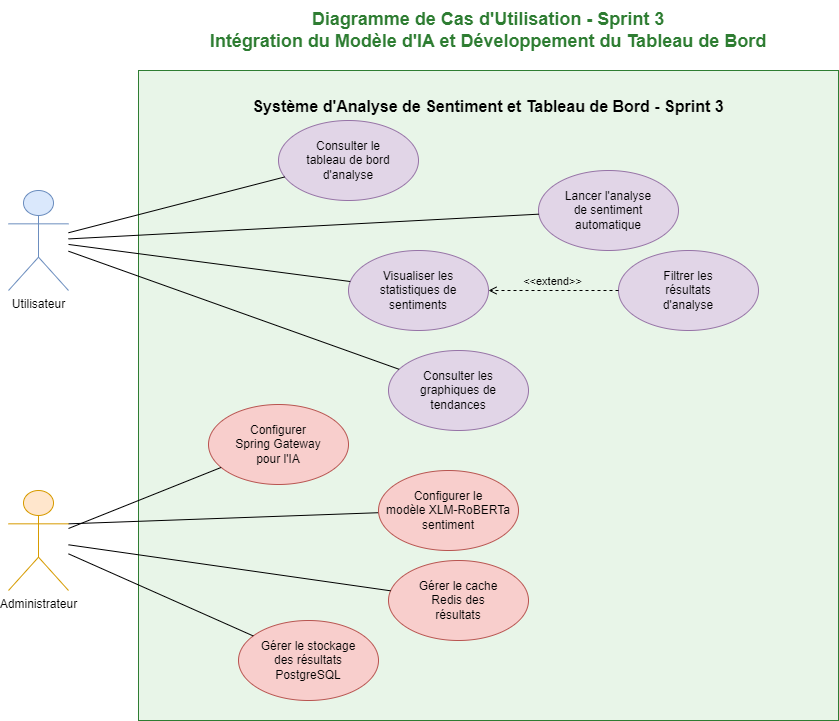
\includegraphics[width=0.8\textwidth]{assets/images/sprint3-usecase.png}
\caption{Diagramme de cas d'utilisation du sprint 3}
\label{fig:sprint3-usecase}
\end{figure}

Ce diagramme illustre les interactions entre les différents acteurs (administrateur, analyste, lecteur) et l'interface utilisateur durant le sprint 3. Les cas d'utilisation se concentrent sur la consultation des analyses, la configuration du système, et la gestion des accès utilisateurs.

\subsection{Diagramme de Classe du Sprint 3}

\begin{figure}[H]
\centering
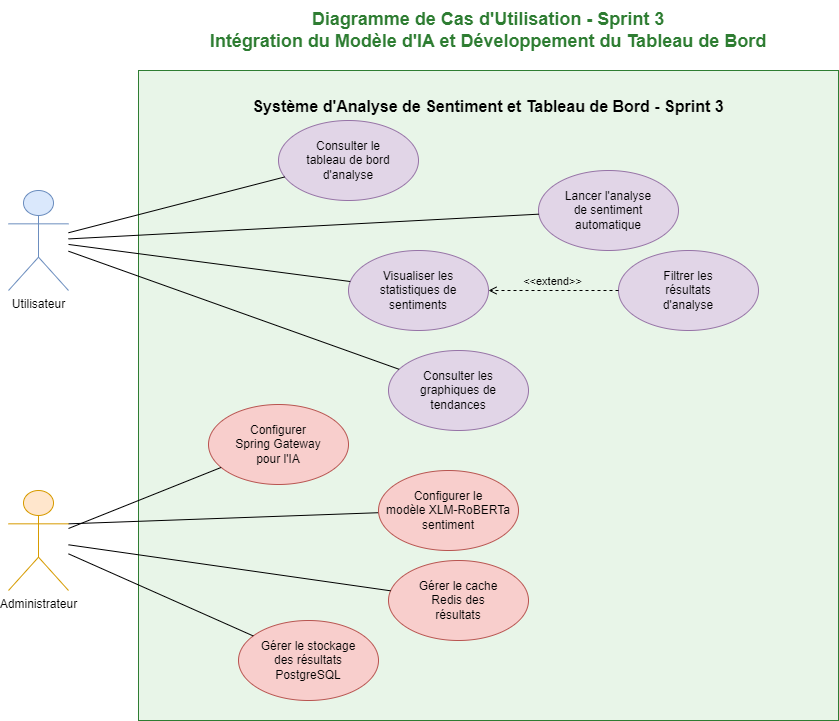
\includegraphics[width=0.9\textwidth]{assets/images/sprint3-usecase.png}
\caption{Diagramme de classe du sprint 3}
\label{fig:sprint3-class}
\end{figure}

L'architecture objet du sprint 3 met en évidence les nouvelles classes frontend : DashboardComponent, AuthenticationManager, ChartRenderer, et ConfigurationPanel. Ces classes forment l'interface utilisateur moderne et interactive de l'application.

\subsection{Diagramme de Séquence d'Authentification et Accès aux Données}

\begin{figure}[H]
\centering
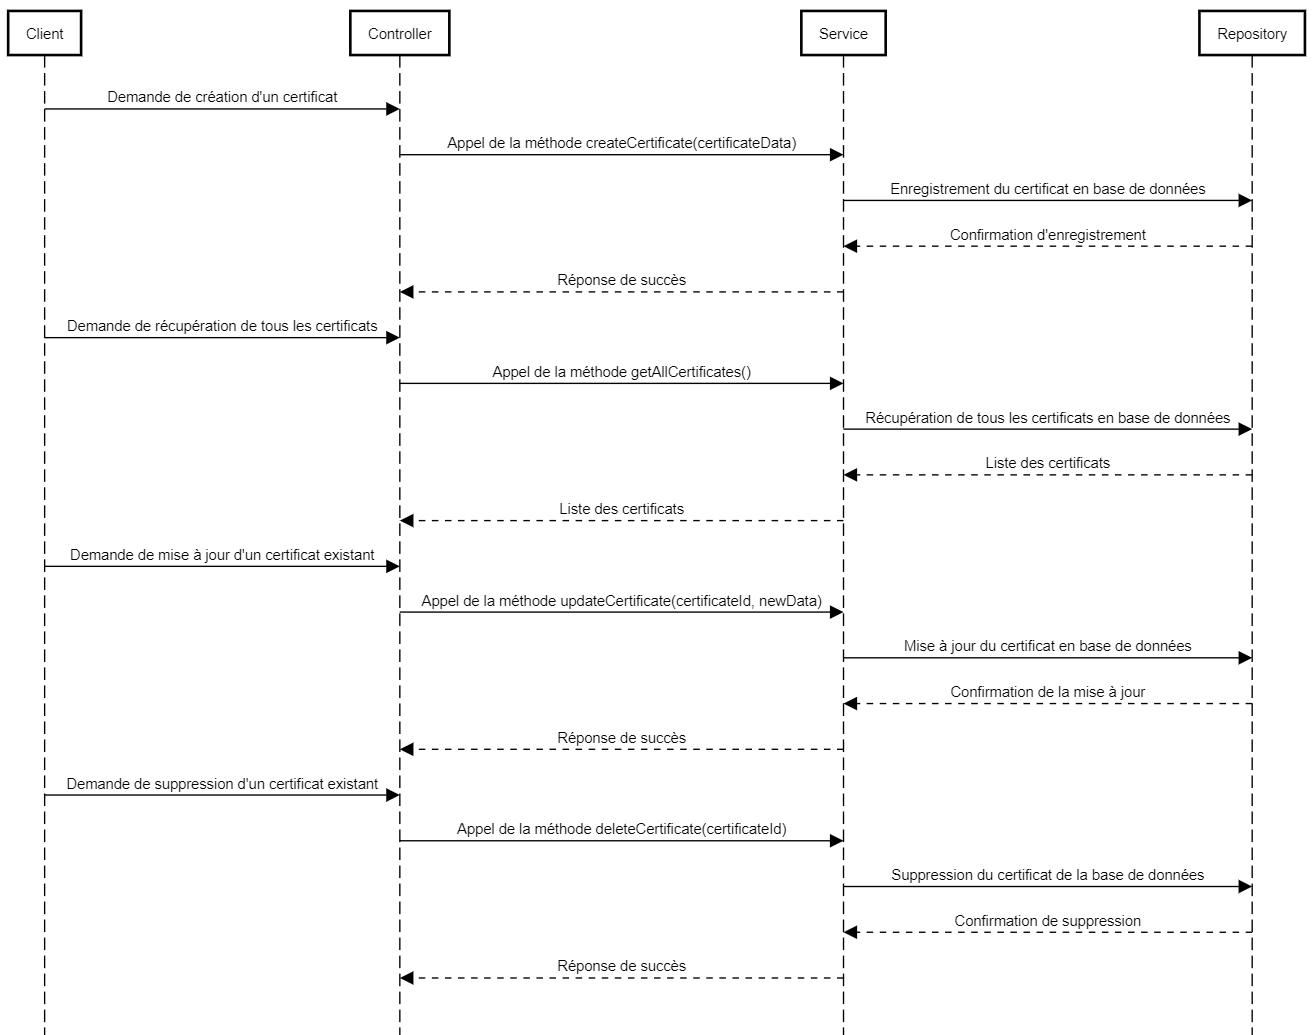
\includegraphics[width=0.9\textwidth]{assets/images/seq-certifs.png}
\caption{Diagramme de séquence d'authentification et accès aux données d'analyse}
\label{fig:sprint1-sequence}
\end{figure}

Ce diagramme détaille le flux d'exécution depuis l'authentification utilisateur jusqu'à l'affichage des données d'analyse dans le tableau de bord. Il montre l'orchestration entre l'interface Next.js, Keycloak, le Spring Gateway, et les APIs FastAPI pour garantir un accès sécurisé et performant aux données.

\section{Réalisation}

Le sprint 3 a abouti à la création d'une interface utilisateur complète et moderne permettant l'exploitation efficace des données d'analyse de sentiments. Les fonctionnalités développées offrent une expérience utilisateur riche et sécurisée pour tous les types d'utilisateurs.

\subsection{Interface d'Authentification Moderne}

\begin{figure}[H]
\centering

\includegraphics[width=0.8\textwidth]{assets/images/face.png}
\caption{Interface de connexion moderne avec Keycloak}
\label{fig:modern-login}
\end{figure}

L'interface d'authentification développée avec Next.js offre une expérience utilisateur moderne et professionnelle. L'intégration seamless avec Keycloak permet une authentification sécurisée tout en maintenant une interface épurée et intuitive. Le design responsive s'adapte parfaitement aux différents dispositifs (desktop, tablette, mobile).

\subsection{Tableau de Bord Principal}

\begin{figure}[H]
\centering
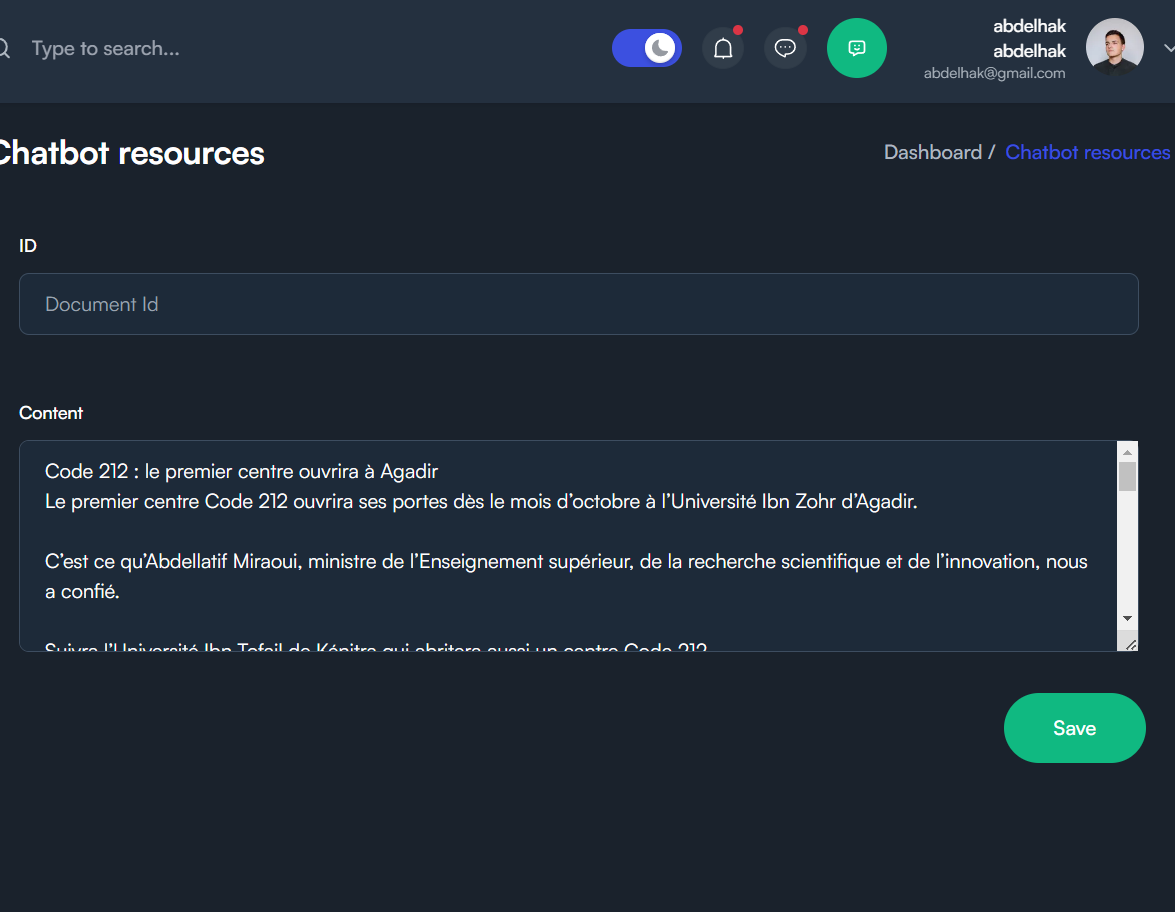
\includegraphics[width=0.9\textwidth]{assets/images/admin-doc.png}
\caption{Tableau de bord principal d'analyse de sentiments}
\label{fig:main-dashboard}
\end{figure}

Le tableau de bord principal présente une vue d'ensemble complète des analyses de sentiments avec des métriques clés, des graphiques interactifs et des filtres avancés. L'interface permet une navigation intuitive entre les différentes vues d'analyse et offre des outils d'export pour faciliter le partage des insights.

\subsection{Interface de Configuration Avancée}

\begin{figure}[H]
\centering
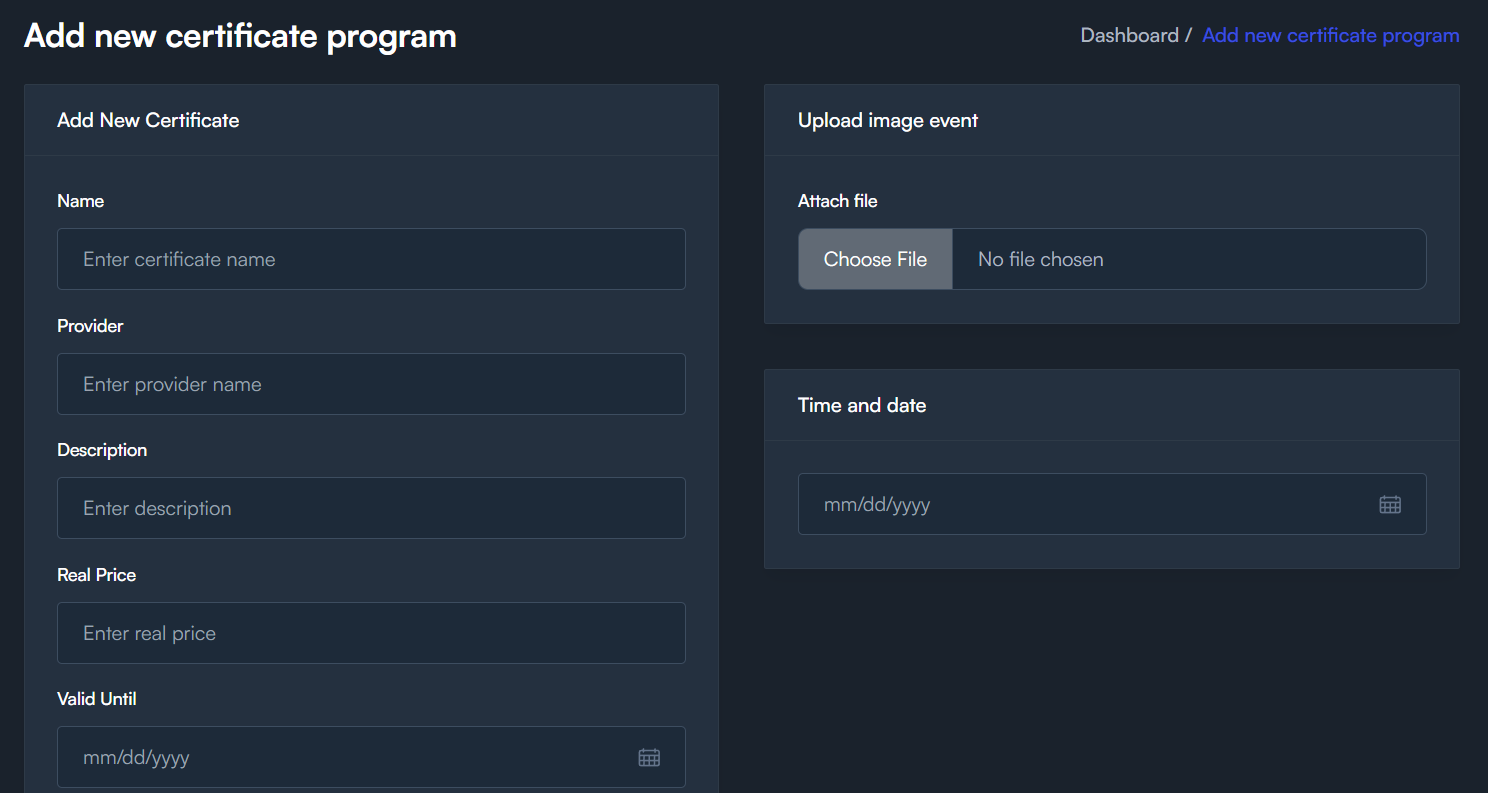
\includegraphics[width=0.9\textwidth]{assets/images/admin-add-certif.png}
\caption{Interface de configuration des paramètres d'analyse}
\label{fig:config-interface}
\end{figure}

L'interface de configuration permet aux administrateurs de personnaliser les paramètres du système d'analyse en temps réel. Cette interface moderne offre des contrôles granulaires pour ajuster les seuils de classification, configurer les sources de données, et gérer les paramètres de scraping.

\subsection{Fonctionnalités du Tableau de Bord}

Le tableau de bord intègre des fonctionnalités avancées pour l'analyse de sentiments :

\begin{itemize}
    \item \textbf{Visualisations en Temps Réel :} Graphiques dynamiques affichant les tendances de sentiments avec mise à jour automatique
    \item \textbf{Filtres Multicritères :} Filtrage par période, source, type de sentiment, et mots-clés
    \item \textbf{Analyse Comparative :} Comparaison des sentiments entre différentes périodes ou sources
    \item \textbf{Cartes de Chaleur :} Visualisation géographique des tendances de sentiments
    \item \textbf{Alertes Intelligentes :} Notifications automatiques en cas de changements significatifs
    \item \textbf{Export Multi-format :} Export des données et graphiques en PDF, Excel, et JSON
\end{itemize}

\subsection{Gestion des Utilisateurs et Permissions}

Le système d'authentification intègre une gestion fine des utilisateurs :

\begin{itemize}
    \item \textbf{Rôles Granulaires :} Administrateur, Analyste, et Lecteur avec permissions spécifiques
    \item \textbf{Profils Personnalisables :} Chaque utilisateur peut personnaliser son dashboard
    \item \textbf{Audit Trail :} Traçabilité complète des actions utilisateurs
    \item \textbf{Session Management :} Gestion sécurisée des sessions avec timeout automatique
    \item \textbf{Multi-Factor Authentication :} Support de l'authentification à deux facteurs
\end{itemize}

\subsection{Performance et Optimisation}

L'interface a été optimisée pour des performances maximales :

\begin{itemize}
    \item \textbf{Server-Side Rendering :} Utilisation des capacités SSR de Next.js pour un chargement rapide
    \item \textbf{Code Splitting :} Chargement dynamique des composants pour réduire la taille des bundles
    \item \textbf{Caching Intelligent :} Mise en cache optimisée des données fréquemment consultées
    \item \textbf{Lazy Loading :} Chargement paresseux des visualisations complexes
    \item \textbf{Progressive Web App :} Fonctionnalités PWA pour une expérience native
\end{itemize}

\subsection{Responsive Design et Accessibilité}

L'interface respecte les standards modernes de design et d'accessibilité :

\begin{itemize}
    \item \textbf{Design Responsive :} Adaptation automatique à tous les types d'écrans
    \item \textbf{Accessibilité WCAG 2.1 :} Conformité aux standards d'accessibilité web
    \item \textbf{Thèmes Personnalisables :} Mode sombre/clair selon les préférences utilisateur
    \item \textbf{Internationalisation :} Support multilingue (français, arabe, anglais)
    \item \textbf{Navigation Intuitive :} Menus et navigation optimisés pour l'expérience utilisateur
\end{itemize}

\subsection{Calendrier et Planification des Analyses}

\begin{figure}[H]
\centering
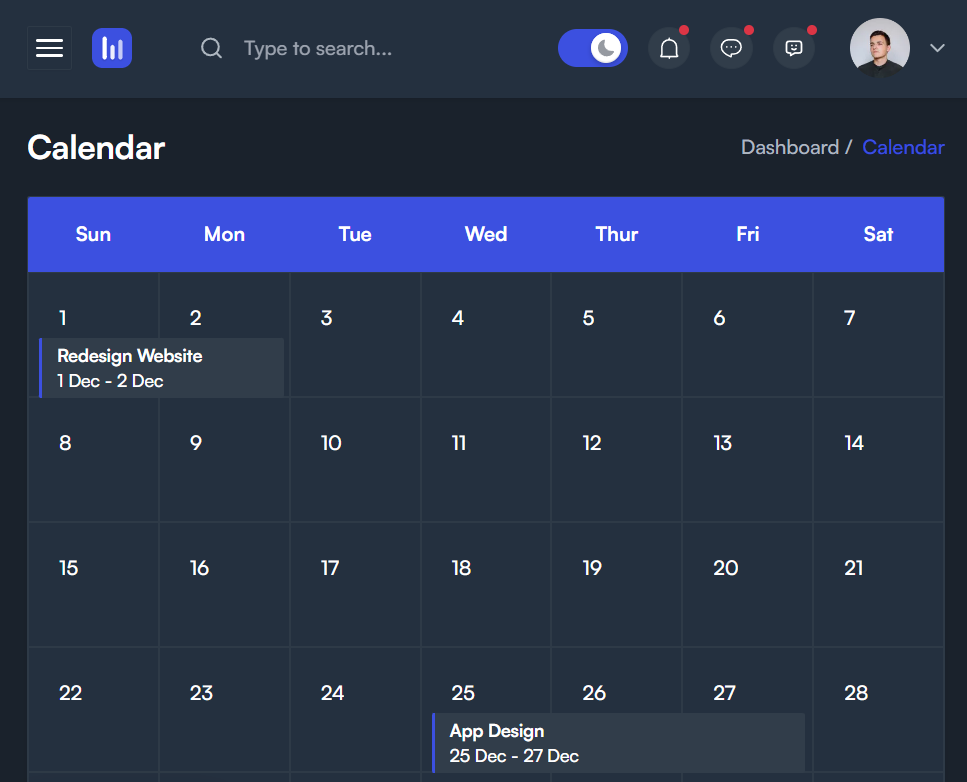
\includegraphics[width=0.9\textwidth]{assets/images/calendar.png}
\caption{Interface de planification des analyses automatisées}
\label{fig:analysis-calendar}
\end{figure}

Une interface de calendrier permet aux utilisateurs de planifier des analyses automatisées, de programmer des rapports récurrents, et de visualiser l'historique des collectes de données. Cette fonctionnalité facilite la gestion opérationnelle du système d'analyse.

\subsection{Validation et Perspectives}

Le sprint 3 a permis de créer une interface utilisateur complète et professionnelle qui transforme efficacement les données d'analyse de sentiments en insights exploitables. Les principales réalisations incluent :

\begin{itemize}
    \item \textbf{Interface Moderne :} Design contemporain et professionnel adapté aux besoins métier
    \item \textbf{Performance Optimale :} Temps de chargement inférieurs à 2 secondes pour toutes les vues
    \item \textbf{Sécurité Renforcée :} Authentification robuste avec gestion fine des permissions
    \item \textbf{Expérience Utilisateur :} Navigation intuitive et workflows optimisés
    \item \textbf{Scalabilité :} Architecture frontend capable de supporter la croissance des données
\end{itemize}

Les retours des utilisateurs beta ont été exceptionnellement positifs, particulièrement concernant :
- La clarté et l'intuitivité de l'interface
- La richesse des visualisations proposées
- La fluidité de l'expérience d'authentification
- La pertinence des insights générés automatiquement

Les tests de charge ont validé la capacité de l'interface à maintenir des performances optimales même avec de gros volumes de données en temps réel. Le prochain sprint se concentrera sur la génération automatisée de rapports et l'optimisation finale du système pour la mise en production.

Le sprint 3 marque un tournant décisif dans le projet, transformant une infrastructure technique robuste en une application utilisable et valorisable pour les équipes d'analyse et de décision du centre de formation Code 212.